\subsection{Mutierende lokale Problemmengen}
\begin{figure}[h]
  \centering
  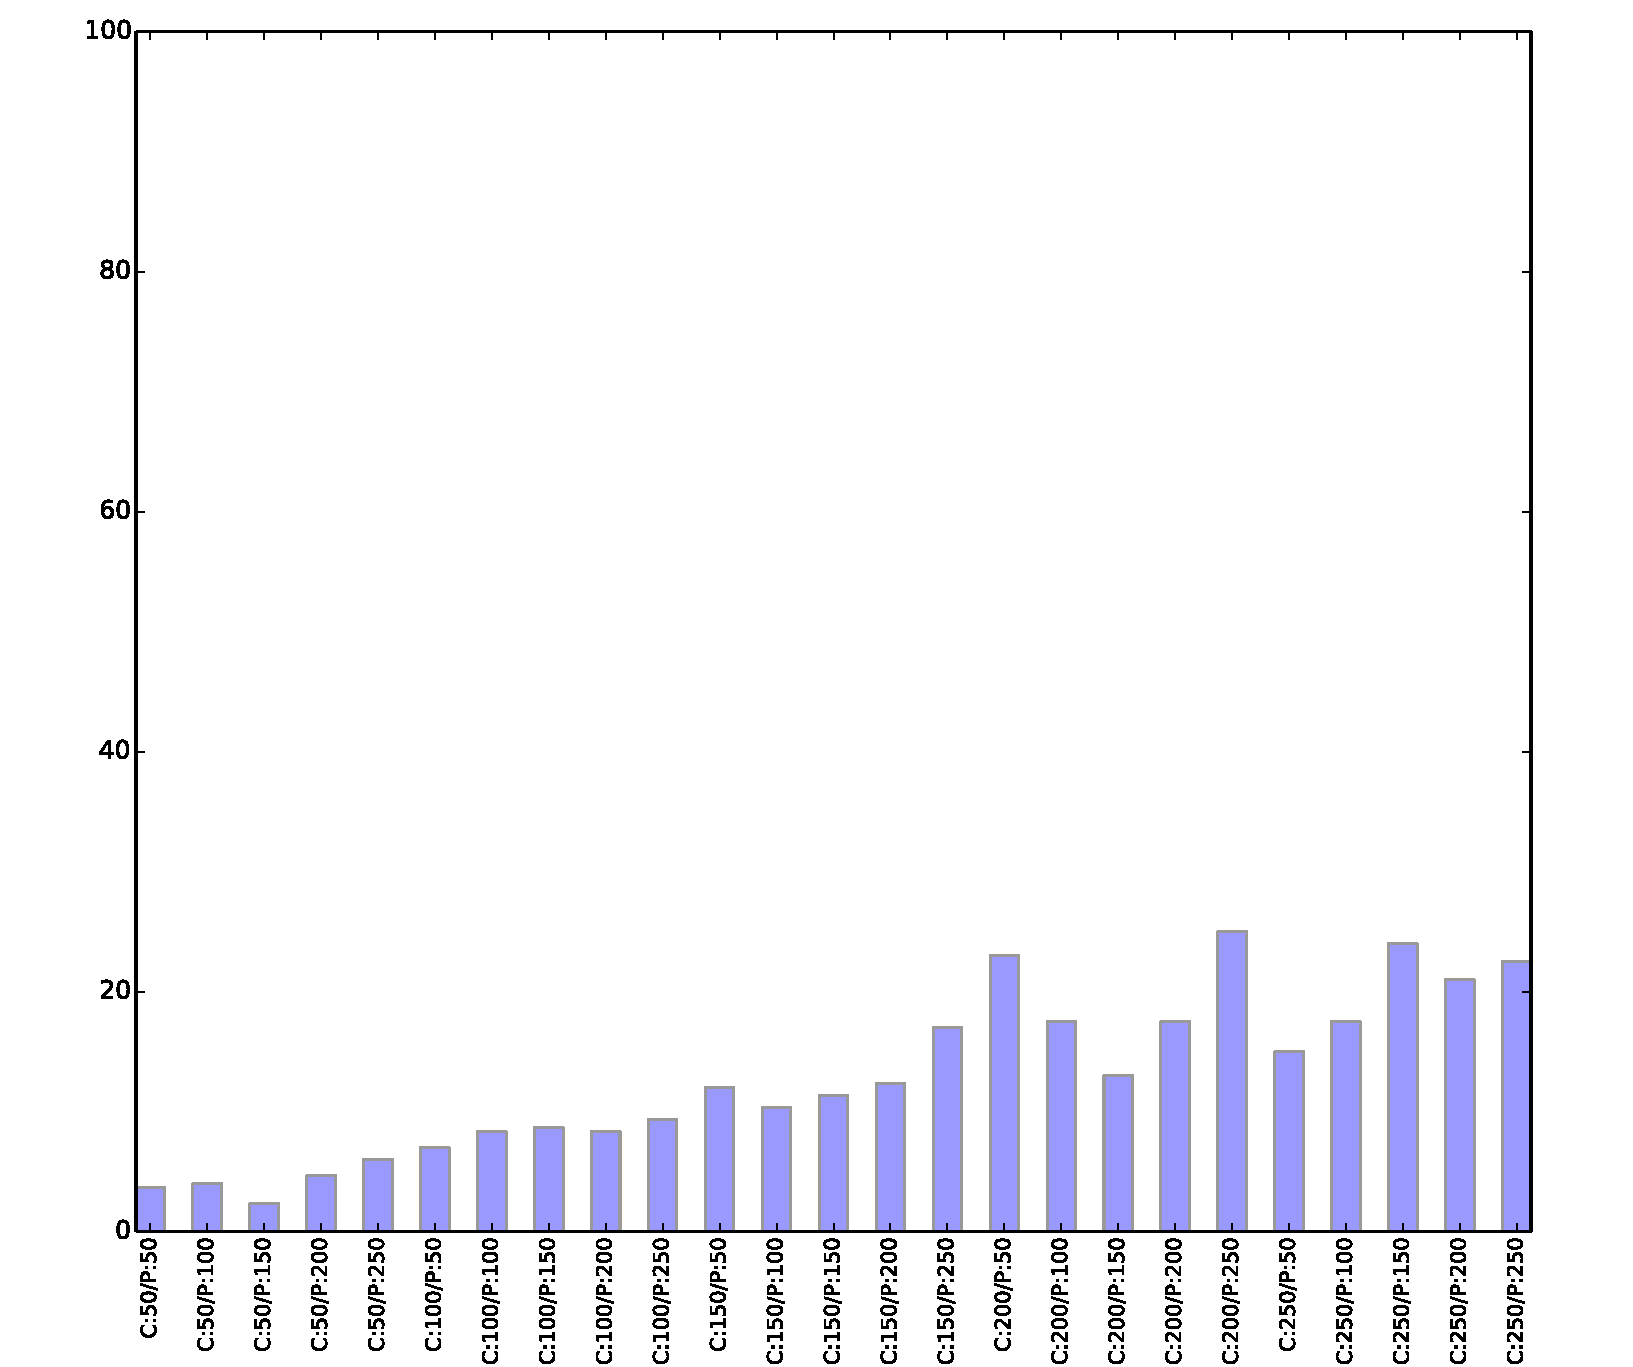
\includegraphics[width=0.75\textwidth]{images/E_L_abab_solved.pdf}
  \caption[ABAB Problem - Lokale mutierende Problemmenge]{ABAB Problem - Lokale mutierende Problemmenge}
  \label{fig:e_l_abab}
\end{figure}

Die Untersuchungen zum Ansatz mit den lokalen Problemmengen, waren ernüchternd. Das Konvergenzverhalten bezüglich Problemmengen- und Populationsgrösse war von der Form her identisch mit demjenigen des Algorithmus mit einer globalen mutierenden Problemmenge. Die Ergebnisse unterschieden sich jedoch dadurch, dass diejenigen mit den lokalen Problemmengen bei gleichen Eingabeparametern schlechter und unregelmässiger waren. Dazu kommt, dass der Rechenaufwand durch den Aufbau des Algorithmus massiv grösser ist als bei den Beiden zuvor untersuchten.

Die Eingabeparameter für die Abbildung \ref{fig:e_l_abab} waren:
\begin{itemize}
	\item Problemmengengrösse: 50, 100, 150, 200, 250
	\item Populationsgrösse: 50, 100, 150, 200, 250
\end{itemize}

Man sieht auch in dieser Grafik erneut eine \flqq Treppenform\frqq auch wenn diese weniger ausgeprägt ist als in Abbildung \ref{fig:e_g_abab}. Weiter fiel auf, dass dieser Algorithmus - wenn er konvergierte - dazu länger brauchte als die Ansätze mit globalen Problemmengen. Länger heisst in diesem Falle, sowohl mehr Zyklen als auch mehr Rechenzeit.